%++++++++++++++++++++++++++++++++++++++++
% Don't modify this section unless you know what you're doing!
\documentclass[letterpaper,12pt]{article}
\usepackage[utf8]{inputenc}
\usepackage[english,russian]{babel}
\usepackage{tabularx} % extra features for tabular environment
\usepackage{amsmath}  % improve math presentation
\usepackage{graphicx} % takes care of graphic including machinery
\usepackage[margin=1in,letterpaper]{geometry} % decreases margins
\usepackage{cite} % takes care of citations
\usepackage[final]{hyperref} % adds hyper links inside the generated pdf file
\hypersetup{
	colorlinks=true,       % false: boxed links; true: colored links
	linkcolor=blue,        % color of internal links
	citecolor=blue,        % color of links to bibliography
	filecolor=magenta,     % color of file links
	urlcolor=blue         
}
%++++++++++++++++++++++++++++++++++++++++


\begin{document}

\title{Исследование ионизационного равновесия газа}
\author{В. Дочкина}
\date{ноябрь 2018}
\maketitle

\begin{abstract}
В данной раб
\end{abstract}


\section{Введение}

The very important physical effect has applications to astronomy, nuclear physics, condensed matter, and more. 


\section{Теория}
\\* Реакция ионизации:
\begin{equation} \label{eq:aperp} % the label is used to reference the equation
A\rightleftharpoons A^{+}+e^{-}
\end{equation}
ЗСМ:
\begin{equation} \label{eq:aperp} % the label is used to reference the equation
m_{a}=m_{i}+m_{e}
\end{equation}
ЗСЭ:
\begin{equation} \label{eq:aperp} % the label is used to reference the equation
E_{0}^{a}=E_{0}^{i}+E_{0}^{e}-I ;§
\end{equation}
где I - потенциал ионизации
\\*
Так как
\begin{equation} \label{eq:aperp} % the label is used to reference the equation
m_{a}\cong m_{i}
\end{equation}
То
\begin{equation} \label{eq:aperp} % the label is used to reference the equation
\lambda_{a}\cong \lambda_{i}
\end{equation} 
Элементарный баланс энергии:
\begin{equation} \label{eq:aperp} % the label is used to reference the equation
\mu_{a}=\mu_{i}+\mu_{e}
\end{equation}
Длина волны де Бройля:
\begin{equation} \label{eq:aperp} % the label is used to reference the equation
\lambda_{b}= \frac{2\pi\hbar}{\sqrt{2\pi m T}}
\end{equation}
Химический потенциал:
\begin{equation} \label{eq:aperp} % the label is used to reference the equation
\mu_{a}=\frac{\partial F_{a}}{\partial N_{a}} ;
\end{equation}
\begin{equation} \label{eq:aperp} % the label is used to reference the equation
F= -Tln{Z} 
\end{equation}
- где F - cвободная энергия; 
\begin{equation} \label{eq:aperp} % the label is used to reference the equation
Z = \frac{z^n}{N!}; z = z_{tr}*z_{in} 
\end{equation}
Используя:
\begin{equation} \label{eq:aperp} % the label is used to reference the equation
F = -Tln{Z}=-Tln{\frac{z^N}{N!}} 
\end{equation}
Получаем:
\begin{equation} \label{eq:aperp} % the label is used to reference the equation
ln{N!}=NlnN-N 
\end{equation}
\begin{equation} \label{eq:aperp} % the label is used to reference the equation
F=T(ln{z^N} - ln{N!})=-T[-NlnN + Nlnz + Nln{e}]= - TNln{\frac{ez}{N}}
\end{equation}
 \begin{equation} \label{eq:aperp} % the label is used to reference the equation
\mu_{a}=\frac{\partial F_a}{\partial N_a}=-T \frac{\partial}{\partial N_a}[\sum N_a ln{\frac{ez_a}{N_a}}]=-T\frac{\partial}{\partial N_a}[\sum N_a ln{\frac{e \not{V} z_{in}}{\lambda{_a}^3_{b}n_a \not{V} }}] 
\end{equation}
\begin{equation} \label{eq:aperp} % the label is used to reference the equation
z_{post}=\frac{V}{\lambda^3_{b}}; n_a=\frac{N_a}{V} 
\end{equation}
\begin{equation} \label{eq:aperp} % the label is used to reference the equation
\mu_a=-T ln{\frac{z_{in}}{\lambda^3_a n_A}}= T ln{\frac{\lambda^3_a n_a}{z{_a}_{in}}} 
\end{equation}
Обозначим:
\begin{equation} \label{eq:aperp} % the label is used to reference the equation
E_{j}-E_{0}=E_{j}^{'}
\end{equation} -энергия относительно основного состояния;
\\*
Тогда:
\begin{equation} \label{eq:aperp} % the label is used to reference the equation
\mu_a = Tln(\frac{\lambda{_a}^3 n_a}{z_{in}*exp(- \frac{E_{a}^{0}}{T})})
\end{equation}
\begin{equation} \label{eq:aperp} % the label is used to reference the equation
\mu_{a}=\mu_{i} + \mu_{e} 
\end{equation}
\begin{equation} \label{eq:aperp} % the label is used to reference the equation
\mu_{a}=Tln{\frac{n_a \lambda_{a}^{3}}{e^{\frac{-E_{a}^{0}}{T}}z_{a}^{'}}} 
\end{equation}
\begin{equation} \label{eq:aperp} % the label is used to reference the equation
\mu_{i}=Tln{\frac{n_i \lambda_{i}^{3}}{e^{\frac{-E_{i}^{0}}{T}}z_{i}^{'}}}
\end{equation}
\begin{equation} \label{eq:aperp} % the label is used to reference the equation
\mu_{e}=Tln{\frac{n_e \lambda_{e}^{3}}{e^{\frac{-E_{e}^{0}}{T}}z_{e}^{'}}}
\end{equation}
-подставим в элементарнтарный баланс энергий:
\begin{equation} \label{eq:aperp} % the label is used to reference the equation
T[ln{\frac{n_a \lambda_{a}^{3}}{e^{\frac{-E_{a}^{0}}{T}}z_{a}^{'}}- ln{\frac{n_i \lambda_{i}^{3}}{e^{\frac{-E_{i}^{0}}{T}}z_{i}^{'}}}} - ln{\frac{n_e \lambda_{e}^{3}}{e^{\frac{-E_{e}^{0}}{T}}z_{e}^{'}}} ]=0 
\end{equation}
\begin{equation} \label{eq:aperp} % the label is used to reference the equation
ln[\frac{n_a \lambda_{a}^{3}* {z}_{i}^{'}{z}_{e}^{'}e^{\frac{-E_{i}^{0}-E_{e}^{0}}{T}}}{e^{\frac{-E_{a}^{0}}{T}}z_{a}^{'}* n_i n_e(\lambda_i \lambda_e)^3}]=0 
\end{equation}
\begin{equation} \label{eq:aperp} % the label is used to reference the equation
(\frac{n_a}{n_i n_e}) \frac{z_{i}^{'}z_{e}^{'}}{z_{a}^{'}}e^\frac{E_{a}^{0}-E_{i}^{0}-E_{e}^{0}}{T}(\frac{\lambda_a}{\lambda_i \lambda_e})^3=1 
\end{equation}
Найдем:
\begin{equation} \label{eq:aperp} % the label is used to reference the equation
\frac{n_e n_i}{n_a}=(\frac{\lambda_a}{\lambda_i \lambda_e})^3\frac{z_{i}^{'}z_{e}^{'}}{z_{a}^{'}}e^{-\frac{I}{T}} 
\end{equation}

\begin{equation} \label{eq:aperp} % the label is used to reference the equation
\lambda_b= \frac{2 \pi \hbar}{\sqrt{2 \pi m T}}
\end{equation}
\begin{equation} \label{eq:aperp} % the label is used to reference the equation
\frac{\lambda_a}{\lambda_i \lambda_e}=\frac{1* \sqrt{m_e} \sqrt{2 \not{m_a} \pi T}}{2 \pi \hbar * \sqrt{\not{m_a}}}= \sqrt{\frac{m_eT}{2 \pi \hbar^2}}
\end{equation}
\begin{equation} \label{eq:aperp} % the label is used to reference the equation
\frac{n_e n_i}{n_a} = (\frac{m_eT}{2 \pi \hbar^2})^{3/2}\frac{z_{i}^{'}z_{e}^{'}}{z_{a}^{'}}e^{-\frac{I}{T}}
\end{equation}
- формула Саха для ионизационного равновесия;
\\*
Введем степень ионизации равную отношению количества ионизированных атомов к общему количеству до ионизации :
\begin{equation} \label{eq:aperp} % the label is used to reference the equation
\alpha= \frac{n_e}{n_e+n_a}
\end{equation}

\begin{equation} \label{eq:aperp} % the label is used to reference the equation
n_e = n_i
\end{equation}

\begin{equation} \label{eq:aperp} % the label is used to reference the equation
n_e + n_i + n_a = n_0,
\end{equation}
где
\begin{equation} \label{eq:aperp} % the label is used to reference the equation
n_0=\frac{P}{T(k_b)}
\end{equation}
- общая концентрация газа;
\begin{equation} \label{eq:aperp} % the label is used to reference the equation
\alpha(n_e+n_a)=n_e
\end{equation}
Выразим концентрации электронов и атомов через степень ионизации и общую концентрацию:

\begin{equation} \label{eq:aperp} % the label is used to reference the equation
n_a=n_0-n_e-n_i
\end{equation}

\begin{equation} \label{eq:aperp} % the label is used to reference the equation
n_e =\alpha(\not{n_e} + n_0 - \not{n_e} - n_i)
\end{equation}
\begin{equation} \label{eq:aperp} % the label is used to reference the equation
n_e = \alpha(n_0 - n_e)
\end{equation}

\begin{equation} \label{eq:aperp} % the label is used to reference the equation
n_e = \frac{\alpha n_0}{1+ \alpha} = \frac{\alpha}{1+\alpha}n_0=n_i
\end{equation}

\begin{equation} \label{eq:aperp} % the label is used to reference the equation
n_a = n_0 - 2n_e = n_0 - \frac{2 \alpha}{1+ \alpha}=n_0(\frac{1 - \alpha}{1 + \alpha })
\end{equation}
В уравнение (29) подставим :
\begin{equation} \label{eq:aperp} % the label is used to reference the equation
\frac{(\frac{\alpha}{1+\alpha})^2n_0^2}{(1-\alpha)(a+\alpha)n_0}=\frac{\alpha^2}{(1-\alpha)(1+\alpha)}n_0=\frac{\alpha^2}{1-\alpha^2}n_0
\end{equation}

\begin{equation} \label{eq:aperp} % the label is used to reference the equation
\frac{\alpha^2}{1-\alpha^2}=(\frac{m_e T}{2 \pi \hbar^2})^{3/2}\frac{2 z_i}{z_a}\frac{T}{P}*e^{-\frac{I}{T}}
\end{equation}
- формула для расчета ионизационного равновесия газа
\section{Покажем, что газ можно считать идеальным}


Don't forget to list all important steps in your experimental procedure!



\section{Analysis}

In this section you will need to show your experimental results. Use tables and
graphs when it is possible. Table~\ref{tbl:bins} is an example.

\begin{table}[ht]
\begin{center}
\caption{Every table needs a caption.}
\label{tbl:bins} % spaces are big no-no withing labels
\begin{tabular}{|cc|} 
\hline
\multicolumn{1}{|c}{$x$ (m)} & \multicolumn{1}{c|}{$V$ (V)} \\
\hline
0.0044151 &   0.0030871 \\
0.0021633 &   0.0021343 \\
0.0003600 &   0.0018642 \\
0.0023831 &   0.0013287 \\
\hline
\end{tabular}
\end{center}
\end{table}

Analysis of equation~\ref{eq:aperp} shows ...

Note: this section can be integrated with the previous one as long as you
address the issue. Here explain how you determine uncertainties for different
measured values. Suppose that in the experiment you make a series of
measurements of a resistance of the wire $R$ for different applied voltages
$V$, then you calculate the temperature from the resistance using a known
equation and make a plot  temperature vs. voltage squared. Again suppose that
this dependence is expected to be linear~\cite{Cyr}, and the proportionality coefficient
is extracted from the graph. Then what you need to explain is that for the
resistance and the voltage the uncertainties are instrumental (since each
measurements in done only once), and they are $\dots$. Then give an equation
for calculating the uncertainty of the temperature from the resistance
uncertainty. Finally explain how the uncertainty of the slop of the graph was
found (computer fitting, graphical method, \emph{etc}.)

If in the process of data analysis you found any noticeable systematic
error(s), you have to explain them in this section of the report.

It is also recommended to plot the data graphically to efficiently illustrate
any points of discussion. For example, it is easy to conclude that the
experiment and theory match each other rather well if you look at
Fig.~\ref{fig:samplesetup} and Fig.~\ref{fig:exp_plots}.

\begin{figure}[ht] 
  \centering
      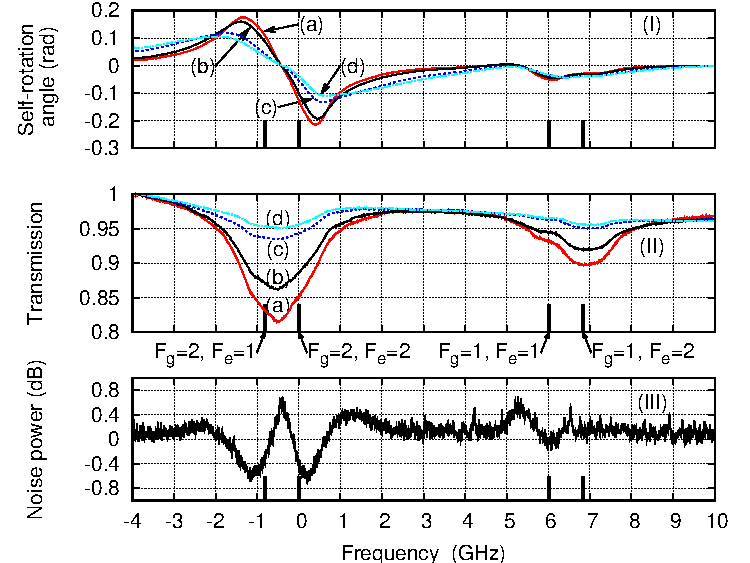
\includegraphics[width=0.5\columnwidth]{sr_squeezing_vs_detuning}

% some figures do not need to be too wide
        \caption{
                \label{fig:exp_plots}  
                Every plot must have axes labeled.
        }
\end{figure}


\section{Conclusions}
Here you briefly summarize your findings.

%++++++++++++++++++++++++++++++++++++++++
% References section will be created automatically 
% with inclusion of "thebibliography" environment
% as it shown below. See text starting with line
% \begin{thebibliography}{99}
% Note: with this approach it is YOUR responsibility to put them in order
% of appearance.

\begin{thebibliography}{99}

\bibitem{melissinos}
A.~C. Melissinos and J. Napolitano, \textit{Experiments in Modern Physics},
(Academic Press, New York, 2003).

\bibitem{Cyr}
N.\ Cyr, M.\ T$\hat{e}$tu, and M.\ Breton,
% "All-optical microwave frequency standard: a proposal,"
IEEE Trans.\ Instrum.\ Meas.\ \textbf{42}, 640 (1993).

\bibitem{Wiki} \emph{Expected value},  available at
\texttt{http://en.wikipedia.org/wiki/Expected\_value}.

\end{thebibliography}


\end{document}
